\documentclass[12pt]{article}
\usepackage[margin=1in]{geometry} 
\usepackage{amsmath,amsthm,amssymb,amsfonts,algpseudocode,graphicx,mathtools}

\newcommand{\N}{\mathbb{N}}
\newcommand{\Z}{\mathbb{Z}}

\newenvironment{problem}[2][Problem]{\begin{trivlist}
\item[\hskip \labelsep {\bfseries #1}\hskip \labelsep {\bfseries #2.}]}{\end{trivlist}}
%If you want to title your bold things something different just make another thing exactly like this but replace ``problem'' with the name of the thing you want, like theorem or lemma or whatever

\newtheorem{theorem}{Theorem}
\newtheorem{lem}{Lemma}
\DeclarePairedDelimiter{\ceil}{\lceil}{\rceil}

\begin{document}

%\renewcommand{\qedsymbol}{\filledbox}
%Good resources for looking up how to do stuff:
%Binary operators: http://www.access2science.com/latex/Binary.html
%General help: http://en.wikibooks.org/wiki/LaTeX/Mathematics
%Or just google stuff

\title{CMPSCI-683 Homework Assignment \#1: Search}
\author{Patrick Pegus II}
\maketitle

\begin{problem}{1}
	Iterative lengthening search is an iterative analogue of uniform-cost search.
	The basic idea is to use increasing limits on path cost.
	If a node is generated whose path cost exceeds the current limit, it is immediately discarded.
	For each new iteration, the limit is set to the lowest path cost of any node discarded in the previous iteration.
	\begin{enumerate}
		\item Show that this algorithm is optimal for general path costs.

			Let modified uniform-cost path search (MUCS) be uniform-cost search (UCS) altered so that it does the following.
			\begin{enumerate}
				\item Discards any generated nodes exceeding the given limit.
				\item Upon failure it returns the lowest path cost of any discarded node or failure if no node was discarded.
			\end{enumerate}
			The function signature of MUCS is:
			\begin{algorithmic}
				\Function{MUCS}{problem, limit}\Return (solution, failure, cost)
				\EndFunction
			\end{algorithmic}
			\begin{lem}
				MUCS is optimal.
			\end{lem}
			\begin{proof}
				Let $p$ be the path returned by MUCS from start state $S$ to goal state $G$.
				Let $C^*$ be the optimal path cost from $S$ to $G$.
				Now suppose that $cost(p) > C^*$.
				Since, like UCS, MUCS expands nodes in order of their optimal path cost, there is only one way this could have happened---
				MUCS must have discarded a generated node representing path $p'$ that is an optimal path or a subpath of an optimal path $p'+p''$.
				But any node discarded by MUCS must have a path cost greater than the limit $l$.
				Since step costs are positive, $cost(p'+p'') > cost(p') > l >= cost(p) > C^*$.
				Therefore, the discarded node could not be an optimal path or a subpath of an optimal path.
			\end{proof}
			Now define iterative lengthening search (ILS) as follows:
			\begin{algorithmic}
				\Function{ILS}{problem}\Return (solution, failure)
					\State $s \gets$ NULL
					\State $f \gets$ NULL
					\State $c \gets 0$
					\While{$s$ is NULL and $f$ is NULL}
						\State $s,f,c \gets$ \Call{MUCS}{problem, $c$}
					\EndWhile
					~\Return $s,f$
				\EndFunction
			\end{algorithmic}
			\begin{theorem}
				ILS is optimal.
			\end{theorem}
			\begin{proof}
				Since ILS only returns solutions returned by MUCS and MUCS is optimal, ILS is optimal.
			\end{proof}
		\item Consider a uniform tree with branching factor b, solution depth d, and unit step costs (each action costs one unit). How many iterations will iterative lengthening require?

			ILS will expand the start state in the first iteration, all states at depth 1 the second iteration, and all states at depth $d$ at iteration $d+1$.
		\item Now consider the case where each step cost is a real number from the interval $[e,1]$ for some $0 < e < 1$. How many iterations are required in the worst case? Try to derive the best estimate you can.

			A worst case example is each step cost along the path to the solution costs 1 and another infinitely long path exists having uniform step cost of $e$.
			In that case ILS will expand the start state the first iteration, all states reachable by a path of cost $e$ the second iteration, $2e$ the third iteration, and the solution having path cost $d$ at iteration $1+\ceil*{\frac{d}{e}}$.
	\end{enumerate}
\end{problem}
\begin{problem}{2}
	Suppose you were doing an A$^*$ search and there were a number of different ways that you could compute an admissible heuristic value.
	Suppose that some were very cheap to compute but also very inaccurate estimators while others were very expensive to compute but were very accurate estimators.
	How would you determine which computation to use for a given application?
	Be as precise as possible.
	Describe intuitively a case in which a fast inaccurate heuristic would be beneficial and a case in which a more time-consuming accurate heuristic would be beneficial.

	\vspace{0.25cm}
	%The time and space complexity of A$^*$ is $O\left(\left(1 + h\right)b^{1+\ceil{\frac{C^*}{\epsilon}}}\right)$ where $h$ is the worst case time to compute the heuristic of a given state,
	%The time and space complexity of A$^*$ is $O\left(b^{1+\ceil{\frac{C^*}{\epsilon}}}\right)$ where 
	%$b$ is the worst case branching factor achieved with the heuristic,	$C^*$ is the optimal solution cost, and $\epsilon > 0$ is the smallest step cost.
	Let $i$ be the fast inaccurate heuristic and $a$ be the expensive accurate heuristic.
	We could say that the average time and space complexity of A$^*$ is $\left(1 + h\right)b^{1+\ceil{\frac{C^*}{e}}}$ where $h$ is the average time to compute the heuristic of a given state,
	$b$ is the effective branching factor achieved with the heuristic,	$C^*$ is the optimal solution cost, and $e$ is the average step cost.
	Therefore, if $C^*$ is much larger than $e$, $b$ should be reduced as much as possible by choosing $a$.
	%Alternatively, if $C^*$ known to be not much greater than $e$ and effective branching factor of the implicit search tree is low (near 2), then $i$ may be acceptable.
	Alternatively, if $C^*$ known to be not much greater than $e$, then $i$ may be acceptable.
	However, if $a$ can be cached and many searches must be computed within the domain, then the cost of computing the $a$ cache can be amortized over all searches making the average time complexity near $b^{1+\ceil{\frac{C^*}{e}}}$.

	Special properties of step cost function can also influence the heuristic choice.
	Suppose paths leading to an optimal solution have decreasing step costs and others do not.
	Then the search space would be self-pruning for A$^*$ even if the given heuristic was 0 for all states.
	Therefore, $i$ would be a good choice, although a greedy search might be a better choice.
	Conversely, $a$ would be required in the reverse situation.

%	Depth of solution.
%	Memory limitations.
%	Time limitations.
%	Cache heuristic for multiple lookups.
%	If states not leading to an optimal solution have larger step costs than those leading to a solution, then the implicit search tree is self-pruning with UCS and an accurate heuristic is not necessary. Parabolic trough path cost
\end{problem}
\begin{problem}{3}
	Give an example of a search space in which A* would expand a node with a g-value that is greater than the cost of the optimal path from the initial state to that state.
	To do that, draw a small graph, designate one node as an initial state and one node as the goal state.
	Assign path costs to edges and an admissible heuristic estimate to each node.
	\begin{enumerate}
		\item Show the graph and trace the execution of A* until it terminates.

			\vspace{0.25cm}
%			If the implementation of A$^*$ has no duplicate node handling, this is impossible.
%			\begin{proof}
%				Let node $n$ represent a path with cost greater than the optimal path cost $C^*$.
%				Let node $n'$ represent an optimal path.
%				For $n$ to be expanded before some node $n'$,
%				\begin{align*}
%					g(n) + h(n) &<= g(n') + h(n') \\
%					g(n) + h(n) &<= g(n') \text{, since the last state in $n'$ is the goal state and $h$ is admissible} \\
%					g(n) + h(n) &<= C^* \\
%					g(n) &<= C^* \text{, assuming that $h$ is non-negative}\\
%				\end{align*}
%			\end{proof}
%			However, if the implementation handles duplicates so that only states and not path costs to reach states are saved in the closed list, then the graph in Figure~\ref{fig:p3graph} will cause the situation described.
%			This execution trace is shown in Table~\ref{tbl:trace}.
			In Figure~\ref{fig:p3graph}, node representing path $(I,C)$ with cost 5 is expanded before the node representing path $(I,A,C)$ with cost 4. The execution trace is shown in Table~\ref{tbl:trace}.
			\begin{figure}[h]
				\centering
				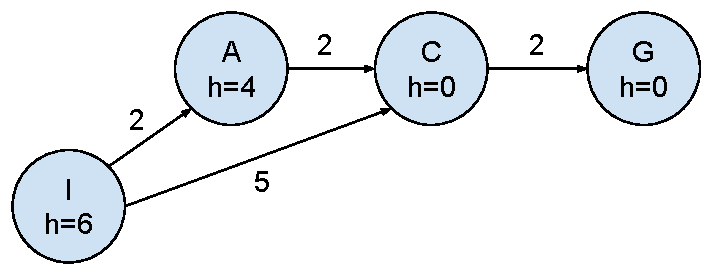
\includegraphics[width=0.8\textwidth]{fig/p3graph.pdf}
				\caption{$I$ and $G$ are the initial and goal states, respectively.}
				\label{fig:p3graph}
			\end{figure} \\
			\begin{table}[h]
				\centering
				%\begin{tabular}{c|c|c}
				\begin{tabular}{c|c}
					Expansion & Open List \\ %& Closed List \\
					\hline
%					1 & $[(I; 0+6)]$ & $[]$ \\
%					2 & $[(I,A; 2+4), (I,C; 5+0)]$ & $[(I,0)]$ \\
%					3 & $[(I,A; 2+4), (I,C,G; 5+2)]$ & $[(I,0),(C,5)]$ \\
%					4 & $[(I,A,C; 4+0), (I,C,G; 5+2)]$ & $[(I,0),(C,4),(A,2)]$ \\
%					5 & $[(I,A,C,G; 6+0), (I,C,G; 5+2)]$ & $[(I,0),(C,4),(A,2),(G,6)]$ \\
%					4 & $[(I,C,G; 5+2)]$ & $[I,C]$ \\
					1 & $[(I; 0+6)]$ \\
					2 & $[(I,C; 5+0), (I,A; 2+4)]$ \\
					3 & $[(I,A; 2+4), (I,C,G; 7+0)]$  \\
					4 & $[(I,A,C; 4+0), (I,C,G; 7+0)]$  \\
					5 & $[(I,A,C,G; 6+0), (I,C,G; 7+0)]$ \\
				\end{tabular}
				\caption{Execution trace of A$^*$ on the graph in Figure~\ref{fig:p3graph}. Nodes are given symbolically as $(path; g+h)$.}% of A$^*$ implemented with duplicate handling that does not remember cost information in the closed list.}
				\label{tbl:trace}
			\end{table}
		\item Is your heuristic function consistent? Is it generally possible to create such an example when the heuristic is consistent? Explain your answer.

			\vspace{0.25cm}
			My heuristic is inconsistent. $h(A) = 4 \nleq cost(A,C) + h(C) = 2$.
\end{enumerate}
\end{problem}

\end{document}
